\documentclass{article}

\usepackage{fancyhdr}
\usepackage{extramarks}
\usepackage{amsmath}
\usepackage{amsthm}
\usepackage{amsfonts}
\usepackage{tikz}
\usepackage{tikz-qtree}
\usepackage[plain]{algorithm}
\usepackage{algpseudocode}
\usepackage{listings}
\usepackage{enumerate}
\lstset{breaklines=true}

\usetikzlibrary{automata,positioning,calc}

%
% Basic Document Settings
%

\topmargin=-0.45in
\evensidemargin=0in
\oddsidemargin=0in
\textwidth=6.5in
\textheight=9.0in
\headsep=0.25in

\linespread{1.1}

\pagestyle{fancy}
\lhead{\hmwkAuthorName}
\chead{\hmwkClass\ (\hmwkClassInstructor): \hmwkTitle}
\rhead{\firstxmark}
\lfoot{\lastxmark}
\cfoot{\thepage}

\renewcommand\headrulewidth{0.4pt}
\renewcommand\footrulewidth{0.4pt}

\setlength\parindent{0pt}

%
% Create Problem Sections
%

\newcommand{\enterProblemHeader}[1]{
    \nobreak\extramarks{}{Problem \arabic{#1} continued on next page\ldots}\nobreak{}
    \nobreak\extramarks{Problem \arabic{#1} (continued)}{Problem \arabic{#1} continued on next page\ldots}\nobreak{}
}

\newcommand{\exitProblemHeader}[1]{
    \nobreak\extramarks{Problem \arabic{#1} (continued)}{Problem \arabic{#1} continued on next page\ldots}\nobreak{}
    \stepcounter{#1}
    \nobreak\extramarks{Problem \arabic{#1}}{}\nobreak{}
}

\newcommand{\bipgraph}[2]{%
    \begin{tikzpicture}[every node/.style={circle,draw}]
    \foreach \xitem in {1,...,#1}
    {%
    % first set
    \node at (0,\xitem) (a\xitem) {};
    % second set
    \node at (2,\xitem) (b\xitem) {};   
    }%

    % connections
    \foreach \x [count=\xi] in {#2}
    {% 
    \foreach \tritem in \x % <-- Here no braces to make it a foreach list also not \xi but \x
    \draw(a\xi) -- (b\tritem);
    }
    \end{tikzpicture}  
}

\newcommand{\bipgraphComplete}[1]{%
    \begin{tikzpicture}[every node/.style={circle,draw}]
    \foreach \xitem in {1,...,#1}
    {%
    % first set
    \node at (0,\xitem) (a\xitem) {};
    % second set
    \node at (2,\xitem) (b\xitem) {};   
    }%

    % connections
    \foreach \x in {1,...,#1}
    {% 
    \foreach \y in {1,...,#1}
        \draw(a\x) -- (b\y);
    }
    \end{tikzpicture}  
}

\setcounter{secnumdepth}{0}
\newcounter{partCounter}
\newcounter{homeworkProblemCounter}
\setcounter{homeworkProblemCounter}{1}
\nobreak\extramarks{Problem \arabic{homeworkProblemCounter}}{}\nobreak{}

%
% Homework Problem Environment
%
% This environment takes an optional argument. When given, it will adjust the
% problem counter. This is useful for when the problems given for your
% assignment aren't sequential. See the last 3 problems of this template for an
% example.
%
\newenvironment{homeworkProblem}[1][-1]{
    \ifnum#1>0
        \setcounter{homeworkProblemCounter}{#1}
    \fi
    \section{Problem \arabic{homeworkProblemCounter}}
    \setcounter{partCounter}{1}
    \enterProblemHeader{homeworkProblemCounter}
}{
    \exitProblemHeader{homeworkProblemCounter}
}

%
% Homework Details
%   - Title
%   - Due date
%   - Class
%   - Section/Time
%   - Instructor
%   - Author
%

\newcommand{\hmwkTitle}{Homework\ \#7}
\newcommand{\hmwkDueDate}{February 18, 2015}
\newcommand{\hmwkClass}{Graph Theory}
\newcommand{\hmwkClassTime}{MWF 9:15}
\newcommand{\hmwkClassInstructor}{Professor McGinley}
\newcommand{\hmwkAuthorName}{Rick Sullivan}

%
% Title Page
%

\title{
    \vspace{2in}
    \textmd{\textbf{\hmwkClass:\ \hmwkTitle}}\\
    \normalsize\vspace{0.1in}\small{Due\ on\ \hmwkDueDate}\\
    \vspace{0.1in}\large{\textit{\hmwkClassInstructor\ \hmwkClassTime}}
    \vspace{3in}
}

\author{\textbf{\hmwkAuthorName}}
\date{}

\renewcommand{\part}[1]{\textbf{\large Part \Alph{partCounter}}\stepcounter{partCounter}\\}

%
% Various Helper Commands
%

% Useful for algorithms
\newcommand{\alg}[1]{\textsc{\bfseries \footnotesize #1}}

% For derivatives
\newcommand{\deriv}[1]{\frac{\mathrm{d}}{\mathrm{d}x} (#1)}

% For partial derivatives
\newcommand{\pderiv}[2]{\frac{\partial}{\partial #1} (#2)}

% Integral dx
\newcommand{\dx}{\mathrm{d}x}

% Alias for the Solution section header
\newcommand{\solution}{\textbf{\large Solution}}

% Probability commands: Expectation, Variance, Covariance, Bias
\newcommand{\E}{\mathrm{E}}
\newcommand{\Var}{\mathrm{Var}}
\newcommand{\Cov}{\mathrm{Cov}}
\newcommand{\Bias}{\mathrm{Bias}}

\begin{document}

\maketitle

\pagebreak

\begin{homeworkProblem}
    Determine all \(r\), \(s\) such that \(K_{r,s}\) is planar.
    \\

    \textbf{Solution}
    \\

    \(K_{r,s}\) is planar whenever either \(r\) or \(s\) is less than or equal to 2.
\end{homeworkProblem}
\begin{homeworkProblem}
    Show that the graph obtained by deleting one edge of \(K_{3,3}\) is planar.
    \\

    \textbf{Solution}

    \begin{proof}
    Removing any edge from \(K_{3,3}\) produces an isomorphism of the same graph.

    \(K_{3,3}\):
    \bipgraphComplete{3}
    Remove any one edge:
    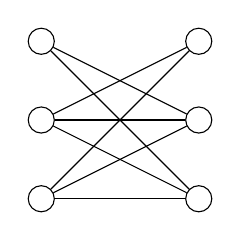
\begin{tikzpicture}[every node/.style={circle,draw}]
    \foreach \xitem in {1,...,3}
    {%
    % first set
    \node at (0,\xitem) (a\xitem) {};
    % second set
    \node at (2,\xitem) (b\xitem) {};   
    }%

    % connections
    \foreach \x in {1,...,3}
    {% 
    \foreach \y in {1,...,2}
        \draw(a\x) -- (b\y);
    }
    \draw(a1) -- (b3);
    \draw(a2) -- (b3);
    \end{tikzpicture}  

    Moving the top and bottom vertices in the left set, we can embed the graph in the plane in the following way

    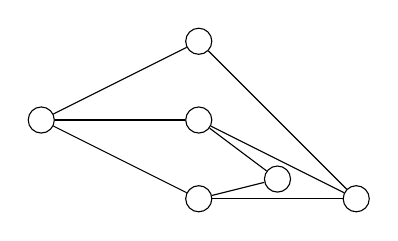
\begin{tikzpicture}[every node/.style={circle,draw}]
    \foreach \xitem in {1,...,3}
    {%
    % first set
    % second set
    \node at (2,\xitem) (b\xitem) {};   
    }%
    \node at (0,2) (a1) {};
    \node at (4,1) (a2) {};
    \node at (3,1.25) (a3) {};

    % connections
    \foreach \x in {1,...,3}
    {% 
    \foreach \y in {1,...,2}
        \draw(a\x) -- (b\y);
    }
    \draw(a1) -- (b3);
    \draw(a2) -- (b3);
    \end{tikzpicture}  
    \end{proof}

\end{homeworkProblem}
\begin{homeworkProblem}
    Determine (using the algorithm given in class) if the graph below is planar. If so, give its planar embedding.
    \\

    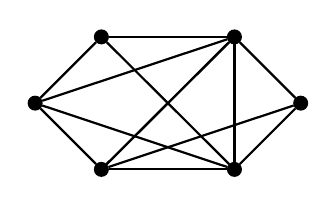
\begin{tikzpicture}[vertex/.style={circle,draw,fill=black,inner sep=0pt,minimum size=5pt}]
        \node[vertex] (a) {};
        \node[vertex] (b) [below left=1cm of a] {};
        \node[vertex] (c) [below right= 1cm of b] {};
        \node[vertex] (d) [right= 1.5cm of a] {};
        \node[vertex] (e) [below right= 1cm of d] {};
        \node[vertex] (f) [below left= 1cm of e] {};

        \path[draw, thick]
        (a) edge node {} (b)
        (b) edge node {} (c)
        (c) edge node {} (d)
        (d) edge node {} (e)
        (e) edge node {} (f)
        (f) edge node {} (a)
        (f) edge node {} (c)
        (c) edge node {} (d)
        (b) edge node {} (f)
        (b) edge node {} (d)
        (d) edge node {} (f)
        (a) edge node {} (d)
        (c) edge node {} (e)
        ;
    \end{tikzpicture}
\end{homeworkProblem}
\begin{homeworkProblem}
    Is the graph below planar? Use one of the theorems we talked about in class, not the algorithm.
    \\
    \usetikzlibrary{shapes.geometric}
    \begin{tikzpicture}[vertex/.style={circle,draw,fill=black,inner sep=0pt,minimum size=5pt}]
        \node[draw=none, regular polygon, regular polygon sides=8, minimum size=2cm] (a) {};
        \node[draw,thick,regular polygon, regular polygon sides=8, minimum size=5cm] (b) {};

        \foreach \x in {1,...,8}{
            \node[vertex] at(a.corner \x) (a\x) {};
            \node[vertex] at(b.corner \x) (b\x) {};
        }

        \foreach \a in {1,...,8} {
            \draw let \n1={int(mod(\a+2,8)+1)} in (a\a)--(a\n1);
            \draw let \n1={int(mod(\a,8)+1)} in (a\a)--(b\n1);
            \draw let \n1={int(mod(\a+6,8)+1)} in (a\a)--(b\n1);
        }
    \end{tikzpicture}
    \\

    \textbf{Solution}
    \begin{proof}
    According to a corollary of Euler's formula, for a graph to be planar, \(e(G) \leq 3n(G)-6\).
    \[
        \begin{split}
            n(G) &= 16\\
            e(G) &= 32\\
            e(G) &\leq 3n(G)-6\\
            32 &\leq 48-6\\
            32 &\leq 42\\
        \end{split}
    \]
    For graphs with no triangular faces, it also must be true that \(e(G) \leq 2n(G)-4\). This graph has no triangular faces, so
    \[
        \begin{split}
            e(G) &\leq 2n(G)-4\\
            32 &\leq 32-4\\
            32 &\leq 28\\
        \end{split}
    \]

    This is not true, so this graph is not planar.
    \end{proof}
\end{homeworkProblem}
\end{document}
